\chapter{Parsing Sintattico}

\section{Per non dimenticare}
    \subsubsection{Context Free}
    Una grammatica libera dal contesto (o non contestuale, context-free o CFG) è una grammatica formale in cui ogni regola sintattica è espressa sotto forma di derivazione di un simbolo a sinistra a partire da uno o più simboli a destra.
    La grammatica formale, nella teoria dei linguaggi formali, è una struttura astratta che descrive un linguaggio formale in modo preciso, è cioè un sistema di regole che delineano matematicamente un insieme (di solito infinito) di sequenze finite di simboli (stringhe) appartenenti ad un alfabeto anch'esso finito.
    \subsubsection{Chomsky Normal Form}
    In formal language theory, a context-free grammar, G, is said to be in Chomsky normal form (first described by Noam Chomsky) if all of its production rules are of the form:
    
        A → BC,   or
        A → a,   or
        S → ε,
    
    where A, B, and C are nonterminal symbols, the letter a is a terminal symbol (a symbol that represents a constant value), S is the start symbol, and ε denotes the empty string. Also, neither B nor C may be the start symbol, and the third production rule can only appear if ε is in L(G), the language produced by the context-free grammar G.
    
    Every grammar in Chomsky normal form is context-free, and conversely, every context-free grammar can be transformed into an equivalent one which is in Chomsky normal form and has a size no larger than the square of the original grammar's size.

\section{CYK: Cocke-Younger-Kasami}
\begin{abstract}
Algoritmo di parsing per grammatiche \textbf{context free}, che utilizza il bottom-up parsing e la programmazione dinamica.
\end{abstract}

\section{Esempio su stringa visto a lezione 31/10/23}

    stringa: "baaba"

    \susubbsection{Regole Grammatica}
        \begin{itemize}
            \item{S -> AB}
            \item{S -> BC}
            \item{A -> BC}
            \item{A -> a}
            \item{B -> BB}
            \item{B -> CC}
            \item{B -> b}
            \item{C -> a}
        \end{itemize}

    \subsubsection{pseudo algoritmo}
    Lungo la diagonale principale inseriamo i simboli che possono generare i terminali sottostanti, (i,i) := terminale[i];
    
    (i,i+1) := combinazioni possibili di (i,i)x(i+1,i+1);
    (i,i+2) := (i,i)x(i+1,i+2) and (i,i+1)x(i+2,i+1);

    
    \begin{figure}
        \centering
        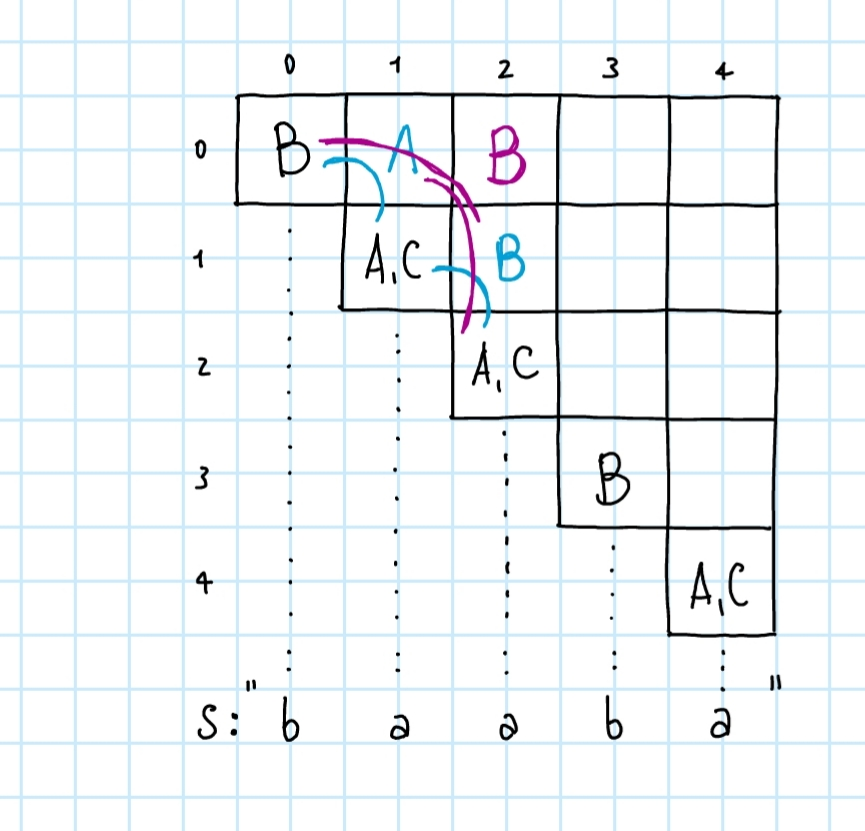
\includegraphics[width=0.5\linewidth]{20231130_165150.jpg}
        \caption{esempio visto a lezione sulla stringa "baaba"}
        \label{fig:enter-label}
        \centering
        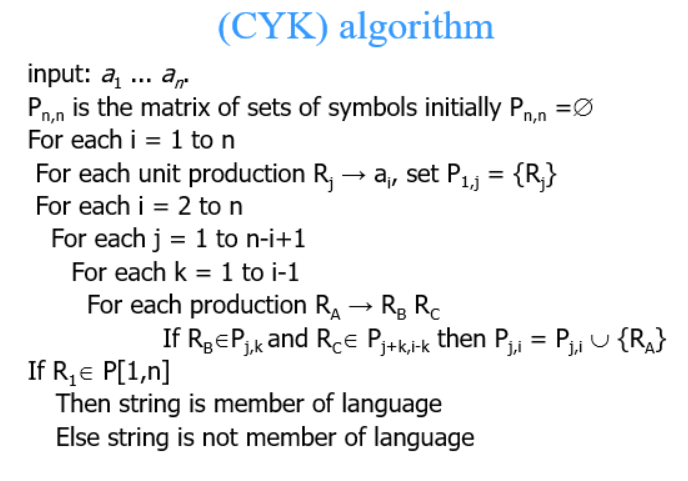
\includegraphics[width=0.5\linewidth]{cyk.PNG}
        \caption{codice algoritmo dalle slides}
        \label{fig:enter-label}
    \end{figure}
    

\section{Classificazione del linguaggio naturale secondo le gerarchie di Chomsky}
\begin{abstract}
L'analisi logica per come la conosciamo non è semplice, non dipende da posizioni (aggettivi prima e dopo il nome) o regole troppo inflessibili... ma anche la stessa tokenizzazione delle 'parole' può presentare problemi ( perchè dividere per spazi? il cinese non divide le parole con spazi ). Invece di cercare una relazione parentetica, guardiamo alle relazioni fra le parole. -> costruzione delle dipendenze
Come definiamo una \textbf{word}?

\begin{Oss}{Esempio:} Il lonfo non vaterca... \end{Oss}
\end{abstract}

